\let\lesson\undefined
\newcommand{\lesson}{\phantomlesson{Bài 2.}}


\setcounter{section}{2}
\section{Bài tập trắc nghiệm}
\begin{enumerate}[label=\bfseries Câu \arabic*:, leftmargin=1.7cm]
	\item \mkstar{1}\\
	Cho hai vật có nhiệt độ khác nhau tiếp xúc với nhau. Nhiệt được truyền từ
	\begin{mcq}
		\item vật có khối lượng lớn hơn sang vật có khối lượng nhỏ hơn.
		\item vật có nhiệt độ cao hơn sang vật có nhiệt độ thấp hơn.
		\item vật ở trên cao sang vật ở dưới thấp.
		\item vật có khối lượng riêng lớn sang vật có khối lượng riêng nhỏ.
	\end{mcq}
\hideall{
\textbf{Đáp án B.}
}

\item \mkstar{1}\\
Người ta cho hai vật dẫn nhiệt A và B tiếp xúc với nhau, sau một thời gian khi có trạng thái cân bằng nhiệt thì hai vật này có
\begin{mcq}(4)
	\item cùng nhiệt độ.
	\item cùng nội năng.
	\item cùng năng lượng.
	\item cùng nhiệt lượng.
\end{mcq}
\hideall{
\textbf{Đáp án A.}
}

\item  \mkstar{1}\\
Đơn vị đo nhiệt độ trong thang nhiệt Celsius là
\begin{mcq}(4)
	\item $\si{\kelvin}$.
	\item $\si{\degree F}$.
	\item $\si{\newton}$.
	\item $\si{\celsius}$.
\end{mcq}
\hideall{
\textbf{Đáp án D.}
}

\item \mkstar{1}\\
Nhiệt kế chất lỏng được chế tạo dựa trên nguyên tắc nào?
\begin{mcq}
	\item Sự nở vì nhiệt của chất lỏng.
	\item Sự phụ thuộc của tốc độ dòng chảy theo nhiệt độ.
	\item Sự thay đổi điện trở của khối chất lỏng theo nhiệt độ.
	\item Sự phụ thuộc của áp suất chất lỏng theo nhiệt độ.
\end{mcq}
\hideall{
\textbf{Đáp án A.}
}

\item Trong các nhiệt kế sau đây, em hãy chọn nhiệt kế phù hợp để đo nhiệt độ của nước đang được đun sôi?
\begin{mcq}
	\item Nhiệt kế y tế có thang chia độ từ $\SI{35}{\celsius}$ đến $\SI{42}{\celsius}$.
	\item Nhiệt kế rượu có thang chia độ từ $\SI{-30}{\celsius}$ đến $\SI{60}{\celsius}$.
	\item Nhiệt kế thuỷ ngân có thang chia độ từ $\SI{-10}{\celsius}$ đến $\SI{110}{\celsius}$.
	\item Nhiệt kế hồng ngoại có thang chia độ từ $\SI{30}{\celsius}$ đến $\SI{45}{\celsius}$.
\end{mcq}
\hideall{
\textbf{Đáp án C.}
}

\item \mkstar{1}\\
Cách xác định nhiệt độ trong thang nhiệt độ Celsius là
\begin{mcq}
	\item Lấy nhiệt độ của nước khi đóng băng là $\left(\SI{10}{\celsius}\right)$ và nhiệt độ sôi của nước $\left(\SI{100}{\celsius}\right)$ làm chuẩn.
	\item Lấy nhiệt độ của nước khi đóng băng là $\left(\SI{100}{\celsius}\right)$ và nhiệt độ sôi của nước $\left(\SI{0}{\celsius}\right)$ làm chuẩn.
	\item Lấy nhiệt độ của nước khi đóng băng là $\left(\SI{0}{\celsius}\right)$ và nhiệt độ sôi của nước $\left(\SI{100}{\celsius}\right)$ làm chuẩn.
	\item Lấy nhiệt độ của nước khi đóng băng là $\left(\SI{100}{\celsius}\right)$ và nhiệt độ sôi của nước $\left(\SI{10}{\celsius}\right)$ làm chuẩn.
\end{mcq}
\hideall{
\textbf{Đáp án C.}
}

\item \mkstar{1}\\
Điểm đóng băng và sôi của nước theo thang Kelvin là
\begin{mcq}(4)
	\item $\SI{0}{\kelvin}$ và $\SI{100}{\kelvin}$.
	\item $\SI{273}{\kelvin}$ và $\SI{373}{\kelvin}$.
	\item $\SI{37}{\kelvin}$ và $\SI{73}{\kelvin}$.
	\item $\SI{32}{\kelvin}$ và $\SI{212}{\kelvin}$.
\end{mcq}
\hideall{
\textbf{Đáp án B.}
}

\item \mkstar{1}\\
Độ không tuyệt đối là nhiệt độ ứng với
\begin{mcq}(4)
	\item $\SI{0}{\kelvin}$.
	\item $\SI{0}{\celsius}$.
	\item $\SI{273}{\kelvin}$.
	\item $\SI{273}{\celsius}$.
\end{mcq}
\hideall{
\textbf{Đáp án A.}
}

\item \mkstar{1}\\
Chọn phát biểu \textbf{đúng}.\\
Nhiệt độ không tuyệt đối là nhiệt độ mà tại đó
\begin{mcq}
	\item chuyển động nhiệt của phân tử hầu như dừng lại.
	\item nước bắt đầu đông thành đá.
	\item tất cả chất khí hoá lỏng.
	\item tất cả chất khí hoá rắn.
\end{mcq}
\hideall{
\textbf{Đáp án A.}
}

\item Không thể dùng nhiệt kế rượu để đo nhiệt độ của nước đang sôi vì
\begin{mcq}(2)
	\item rượu sôi ở nhiệt độ cao hơn $\SI{100}{\celsius}$.
	\item rượu sôi ở nhiệt độ thấp hơn $\SI{100}{\celsius}$.
	\item rượu đông đặc ở nhiệt độ $\SI{100}{\celsius}$.
	\item rượu đông đặc ở nhiệt độ thấp hơn $\SI{0}{\celsius}$.
\end{mcq}
\hideall{
\textbf{Đáp án B.}
}

\item Biểu thức nào sau đây là đúng khi biến đổi nhiệt độ từ thang Celsius sang thang Kelvin?
\begin{mcq}(2)
	\item $T\left(\si{\kelvin}\right)=t\left(\si{\celsius}\right)-273$.
	\item $T\left(\si{\kelvin}\right)=t\left(\si{\celsius}\right)+273$.
	\item $T\left(\si{\kelvin}\right)=\dfrac{t\left(\si{\celsius}\right)+273}{2}$.
	\item $T\left(\si{\kelvin}\right)=2t\left(\si{\celsius}\right)+273$.
\end{mcq}
\hideall{
\textbf{Đáp án B.}
}

\item \mkstar{2}\\
Cho các bước như sau:
\begin{enumerate}[label=(\arabic*)]
	\item Thực hiện phép đo nhiệt độ.
	\item Ước lượng nhiệt độ của vật.
	\item Hiệu chỉnh nhiệt kế.
	\item Lựa chọn nhiệt kế phù hợp.
	\item Đọc và ghi kết quả đo.
\end{enumerate}
Các bước đúng khi thực hiện đo nhiệt độ của một vật là
\begin{mcq}(2)
	\item (2), (4), (3), (1), (5).
	\item (1), (4), (2), (3), (5).
	\item (1), (2), (3), (4), (5).
	\item (3), (2), (4), (1), (5).
\end{mcq}
\hideall{
\textbf{Đáp án A.}
}

\item \mkstar{2}\\
Nhiệt độ trung bình của nước ở thang nhiệt độ Celsius là $\SI{27}{\celsius}$ ứng với thang nhiệt độ Kelvin thì nhiệt độ của nước là
\begin{mcq}(4)
	\item $\SI{273}{\kelvin}$.
	\item $\SI{300}{\kelvin}$.
	\item $\SI{246}{\kelvin}$.
	\item $\SI{327}{\kelvin}$.
\end{mcq}
\hideall{
\textbf{Đáp án B.}\\
$$T=t+273=\SI{300}{\kelvin}.$$
}

\item \mkstar{2}\\
Nhiệt độ mùa đông tại thành phố New York (Mỹ) là $\SI{283}{\kelvin}$, ứng với nhiệt giai Celsius thì nhiệt độ ở đó là
\begin{mcq}(4)
	\item $\SI{10}{\celsius}$.
	\item $\SI{-10}{\celsius}$.
	\item $\SI{5}{\celsius}$.
	\item $\SI{-5}{\celsius}$.
\end{mcq}
\hideall{
\textbf{Đáp án A.}\\
$$t=T-273=\SI{10}{\celsius}.$$
}

\item \mkstar{2}\\
Nhiệt độ vào một ngày mùa hè ở thành phố Hồ Chí Minh là $\SI{35}{\celsius}$. Nhiệt độ đó tương ứng với bao nhiêu độ $\si{\degree F}$?
\begin{mcq}(4)
	\item $\SI{59}{\degree F}$.
	\item $\SI{67}{\degree F}$.
	\item $\SI{95}{\degree F}$.
	\item $\SI{76}{\degree F}$.
\end{mcq}
\hideall{
\textbf{Đáp án C.}\\
$$t\left(\si{\degree F}\right)=32+1,8t\left(\si{\celsius}\right)=\SI{95}{\degree F}.$$
}

\item \mkstar{2}\\
Giá trị nhiệt độ đo được theo thang nhiệt độ Kelvin là $\SI{293}{\kelvin}$. Tính theo thang nhiệt độ Fahrenheit, nhiệt độ đó có giá trị là
\begin{mcq}(4)
	\item $\SI{20}{\degree F}$.
	\item $\SI{100}{\degree F}$.
	\item $\SI{68}{\degree F}$.
	\item $\SI{261}{\degree F}$.
\end{mcq}
\hideall{
\textbf{Đáp án C.}\\
$$t\left(\si{\celsius}\right)=T-273=\SI{20}{\celsius}.$$
$$t\left(\si{\degree F}\right)=32+1,8t\left(\si{\celsius}\right)=\SI{68}{\degree F}.$$
}

\item \mkstar{3}\\
$\SI{104}{\degree F}$ ứng với bao nhiêu độ Kelvin?
\begin{mcq}(4)
	\item $\SI{313}{\kelvin}$.
	\item $\SI{298}{\kelvin}$.
	\item $\SI{328}{\kelvin}$.
	\item $\SI{293}{\kelvin}$.
\end{mcq}
\hideall{
\textbf{Đáp án A.}\\
$$\dfrac{t\left(\si{\degree F}\right)-32}{212-32}=\dfrac{T\left(\si{\kelvin}\right)-273}{373-273}$$
Thay $t\left(\si{\degree F}\right)=\SI{104}{\degree F}$, thu được $T=\SI{313}{\kelvin}.$
}

\item \mkstar{3}\\
Một thang đo $X$ lấy điểm đóng băng là $-10X$, lấy điểm sôi là $90X$. Nhiệt độ của một vật đọc được trên theo nhiệt giai Celsius là $\SI{40}{\celsius}$ thì trong nhiệt giai $X$ có nhiệt độ bằng
\begin{mcq}(4)
	\item $20X$.
	\item $30X$.
	\item $40X$.
	\item $50X$.
\end{mcq}
\hideall{
\textbf{Đáp án B.}\\
Độ chênh lệch nhiệt độ tại điểm băng và điểm sôi trong thang X cũng là 100. Như vậy $\SI{1}{\celsius}$ tương ứng với $\SI{1}{X}$ và
$$t\left(\si{\celsius}\right)=t\left(\si{X}\right)+10.$$
}

\item\mkstar{3}\\
Giả sử có một thang nhiệt độ kí hiệu Z. Nhiệt độ sôi của nước theo thang này là $60Z$, điểm ba cả nước là $-15Z$. Nhiệt độ của vật theo thang Fahrenheit là bao nhiêu nếu nhiệt độ trong thang Z là $-96Z$?
\begin{mcq}(4)
	\item $\SI{-62.4}{\degree F}$.
	\item $\SI{162.4}{\degree F}$.
	\item $\SI{-162.4}{\degree F}$.
	\item $\SI{62.4}{\degree F}$.
\end{mcq}
\hideall{
\textbf{Đáp án C.}\\
$$\dfrac{t\left(\si{\degree F}\right)-32}{212-32}=\dfrac{Z-\left(-15\right)}{60-\left(-15\right)}$$
Thay $Z=-96$ ta thu được $t\left(\si{\degree F}\right)=\SI{-162.4}{\degree F}.$
}

\item\mkstar{3}\\
Hình dưới thể hiện nhiệt kế đo nhiệt độ của một vật. Sai số dụng cụ được lấy bằng một nửa độ chia nhỏ nhất. Kết quả đo nhiệt độ của vật này là
\begin{center}
	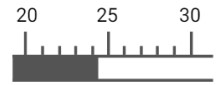
\includegraphics[width=0.25\linewidth]{../figs/VN12-Y24-PH-SYL-002P-3}
\end{center}
\begin{mcq}(4)
	\item $t=\xsi{24.0\pm0.5}{\celsius}$.
	\item $t=\xsi{25.0\pm0.5}{\celsius}$.
	\item $t=\xsi{24.0\pm1.0}{\celsius}$.
	\item $t=\xsi{25.0\pm1.0}{\celsius}$.
\end{mcq}
\hideall{
\textbf{Đáp án A.}
}

\item \mkstar{3}\\
Chiều dài của phần thuỷ ngân trong nhiệt kế là $\SI{2}{\centi\meter}$ ở $\SI{0}{\celsius}$ và $\SI{22}{\centi\meter}$ ở $\SI{100}{\celsius}$. Nhiệt độ là bao nhiêu nếu chiều dài của thuỷ ngân là $\SI{8}{\centi\meter}$?
\begin{mcq}(4)
	\item $\SI{40}{\celsius}$.
	\item $\SI{50}{\celsius}$.
	\item $\SI{20}{\celsius}$.
	\item $\SI{30}{\celsius}$.
\end{mcq}
\hideall{
\textbf{Đáp án D.}\\
$$\dfrac{\ell-\ell_0}{t-t_0}=\dfrac{\ell'-\ell_0}{t'-t_0}$$
$$\Leftrightarrow\dfrac{\SI{22}{\centi\meter}-\SI{2}{\centi\meter}}{\SI{100}{\celsius}-\SI{0}{\celsius}}=\dfrac{\SI{8}{\centi\meter}-\SI{2}{\centi\meter}}{t'-\SI{0}{\celsius}}\Rightarrow t'=\SI{30}{\celsius}.$$
}


\item \mkstar{3}\\
Chiều dài của phần thuỷ ngân trong nhiệt kế là $\SI{2}{\centi\meter}$ ở $\SI{0}{\celsius}$ và $\SI{22}{\centi\meter}$ ở $\SI{100}{\celsius}$. Chiều dài của phần thuỷ ngân sẽ là bao nhiêu nếu nhiệt độ là $\SI{50}{\celsius}$?
\begin{mcq}(4)
	\item $\SI{10}{\centi\meter}$.
	\item $\SI{12}{\centi\meter}$.
	\item $\SI{14}{\centi\meter}$.
	\item $\SI{16}{\centi\meter}$.
\end{mcq}
\hideall{
\textbf{Đáp án B.}\\
$$\dfrac{\ell-\ell_0}{t-t_0}=\dfrac{\ell'-\ell_0}{t'-t_0}$$
$$\Leftrightarrow\dfrac{\SI{22}{\centi\meter}-\SI{2}{\centi\meter}}{\SI{100}{\celsius}-\SI{0}{\celsius}}=\dfrac{\ell'-\SI{2}{\centi\meter}}{\SI{50}{\celsius}-\SI{0}{\celsius}}\Rightarrow \ell'=\SI{12}{\centi\meter}.$$

}

\item \mkstar{3}\\
Sự phụ thuộc vào nhiệt độ của bước sóng điện từ theo hệ thức Wien: $T\cdot\lambda_\text{max}=\SI{2900}{\left(\micro\meter\cdot\kelvin\right)}$ được dùng vào việc chế tạo các nhiệt kế thường dùng hằng ngày như
nhiệt kế hồng ngoại, cũng như các nhiệt kế trong thiên văn để đo nhiệt độ bề mặt của
các thiên thể. Xét một nhiệt kế hồng ngoại khi đo nhiệt độ cơ thể người như hình vẽ.
Bước sóng hồng ngoại do cơ thể người phát ra bằng xấp xỉ bằng
\begin{center}
	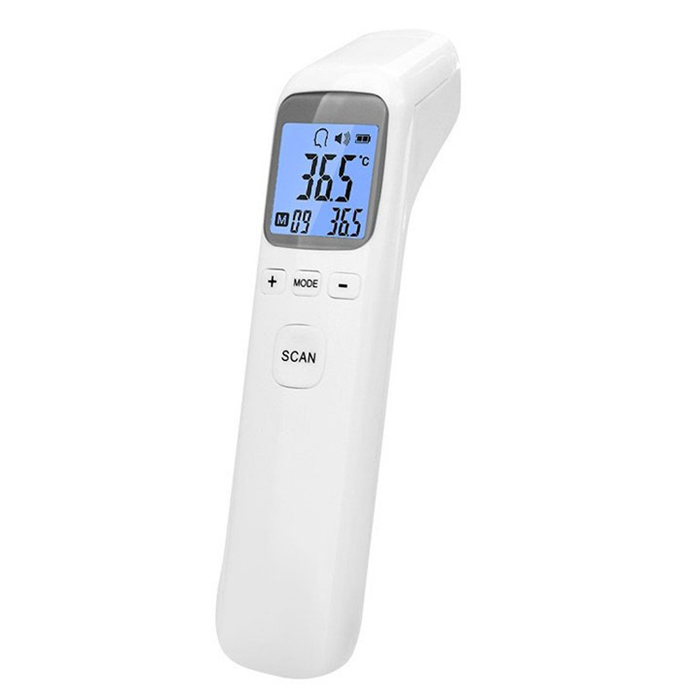
\includegraphics[width=0.3\linewidth]{../figs/VN12-Y24-PH-SYL-002P-1}
\end{center}
\begin{mcq}(4)
	\item $\SI{9.4}{\micro\meter}$.
	\item $\SI{79}{\micro\meter}$.
	\item $\SI{29}{\micro\meter}$.
	\item $\SI{10.6}{\micro\meter}$.
\end{mcq}
\hideall{
\textbf{Đáp án A.}\\
$$\lambda_\text{max}=\dfrac{\SI{2900}{\micro\meter\cdot\kelvin}}{T}=\dfrac{\SI{2900}{\micro\meter\cdot\kelvin}}{36,5+\SI{273}{\kelvin}}\approx\SI{9.4}{\micro\meter}.$$
}

\end{enumerate}
\section{Trắc nghiệm đúng/ sai}
\begin{enumerate}[label=\bfseries Câu \arabic*:, leftmargin=1.7cm]
	\item \mkstar{1}\\
	Bảng sau đây ghi sự thay đổi nhiệt độ của không khí theo thời gian dựa trên số liệu của một trạm khí tượng ở Hà Nội ghi được vào một ngày mùa đông.
	\begin{center}
		\begin{tabular}{|C{8em}|C{1.5em}|C{1.5em}|C{1.5em}|C{1.5em}|C{1.5em}|C{1.5em}|C{1.5em}|C{1.5em}|}
			\hline
			\thead{Thời gian (giờ)}& 1 & 4 & 7 & 10 & 13 & 16 & 19 & 22\\
			\hline
			\thead{Nhiệt độ $\left(\si{\celsius}\right)$} & 13 & 13 &13 & 18& 18 & 20 & 17 & 12\\
			\hline
		\end{tabular}
	\end{center}
\begin{enumerate}[label=\alph*)]
	\item Nhiệt độ lúc 4 giờ là $\SI{286}{\kelvin}$.
	\item Nhiệt độ thấp nhất trong ngày là vào lúc 1 giờ.
	\item Nhiệt độ cao nhất trong ngày là vào lúc 16 giờ.
	\item Độ chênh lệch nhiệt độ trong ngày là $\SI{6}{\celsius}$.
\end{enumerate}
\hideall{
\begin{enumerate}[label=\alph*)]
	\item Đúng.
	\item Sai. Nhiệt độ thấp nhất là $\SI{12}{\celsius}$ vào lúc $\SI{22}{\hour}$.
	\item Đúng.
	\item Sai. Độ chênh lệch nhiệt độ trong ngày là $\SI{8}{\celsius}$.
\end{enumerate}

}

\item \mkstar{2}\\
Bảng dưới đây ghi tên các loại nhiệt kế và thang đo của chúng
\begin{center}
	\begin{tabular}{|C{5cm}|C{6cm}|}
		\hline
		\thead{Loại nhiệt kế} & \thead{Thang nhiệt độ}\\
		\hline
		Thuỷ ngân & Từ $\SI{-10}{\celsius}$ đến $\SI{110}{\celsius}$\\
		\hline
		Rượu & Từ $\SI{-30}{\celsius}$ đến $\SI{60}{\celsius}$\\
		\hline
		Kim loại & Từ $\SI{0}{\celsius}$ đến $\SI{400}{\celsius}$\\
		\hline
		Điện tử & Từ $\SI{34}{\celsius}$ đến $\SI{42}{\celsius}$\\
		\hline
	\end{tabular}
\end{center}
\begin{enumerate}[label=\alph*)]
	\item Dùng nhiệt kế kim loại để đo nhiệt độ nước sôi.
	\item Dùng nhiệt kế điện tử để đo nhiệt độ cơ thể người.
	\item Dùng nhiệt kế thuỷ ngân để đo nhiệt độ không khí trong phòng.
	\item Dùng nhiệt kế rượu để đo nhiệt độ bề mặt bàn là.
\end{enumerate}
\hideall{
\begin{enumerate}[label=\alph*)]
	\item Đúng.
	\item Đúng.
	\item Đúng.
	\item Sai.
\end{enumerate}
}

\item \mkstar{2}\\
Hình bên là một nhiệt kế rượu.
\begin{center}
	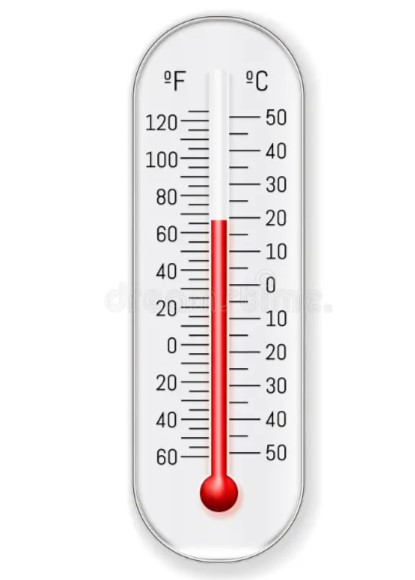
\includegraphics[width=0.25\linewidth]{../figs/VN12-Y24-PH-SYL-002P-2}
\end{center}
\begin{enumerate}[label=\alph*)]
	\item Giới hạn đo của nhiệt kế là $\SI{120}{\celsius}$.
	\item Độ chia nhỏ nhất của nhiệt kế là $\SI{5}{\celsius}$.
	\item Nhiệt độ hiện tại trên nhiệt kế là $\SI{19}{\celsius}$.
	\item Có thể dùng nhiệt kế để xác định nhiệt độ của nước sôi.
\end{enumerate}
\hideall{
\begin{enumerate}[label=\alph*)]
	\item Sai. Giới hạn đo của nhiệt kế là $\SI{50}{\celsius}$.
	\item Đúng.
	\item Sai. ĐCNN của nhiệt kế là $\SI{5}{\celsius}$ nên không thể đọc được giá trị $\SI{19}{\celsius}$, nhiệt độ hiện tại có thể đọc từ nhiệt kế là $\SI{20}{\celsius}$.
	\item Sai. Giới hạn đo của nhiệt kế nhỏ hơn nhiệt độ nước sôi.
\end{enumerate}
}


\end{enumerate}

\section{Bài tập tự luận}
\begin{enumerate}[label=\bfseries Câu \arabic*:, leftmargin=1.7cm]
	\item\mkstar{2}\\
	 Theo dự báo thời tiết ngày 17/04/2024 thì nhiệt độ trung bình ngày - đêm trong
	ngày hôm đó tại Thành phố Hồ Chí Minh là  $\SI{35}{\celsius}-\SI{25}{\celsius}$. Sự chênh lệch nhiệt độ này trong thang đo Kelvin là bao nhiêu $\si{\kelvin}$?
	\hideall{
$$\Delta T=\SI{10}{\kelvin}.$$	
}

\item\mkstar{2}\\ 
Thế giới từng ghi nhận sự thay đổi nhiệt độ rất lớn diễn ra ở Spearfish, South Dakota vào ngày 22/01/1943. Lúc 7h30 sáng, nhiệt độ ngoài trời là $\SI{-20}{\celsius}$. Hai phút sau, nhiệt độ ngoài trời tăng lên đến $\SI{7.2}{\celsius}$. Xác định độ tăng nhiệt độ trung bình trong 2 phút đó theo đơn vị Kelvin/giây.
\hideall{
$$\dfrac{\Delta T}{t}=\dfrac{\SI{27.2}{\kelvin}}{\SI{120}{\second}}\approx\SI{0.23}{\kelvin/\second}.$$
}
\item \mkstar{2}\\
Ở $\SI{20}{\celsius}$ một thanh nhôm dài $\SI{12}{\meter}$. Tính nhiệt độ cần thiết để chiều dài thanh nhôm là $\SI{12.01}{\meter}$. Biết rằng khi nhiệt độ tăng thêm $\SI{1}{\celsius}$ thì thanh nhôm dài thêm $\SI{2.3E-5}{}$ chiều dài ban đầu.
\hideall{
$$\Delta\ell=\alpha\ell_0\Delta t$$
với $\alpha=\SI{2.3E-5}{\kelvin^{-1}}$.
$$\Rightarrow \Delta t=\dfrac{\Delta \ell}{\alpha\ell_0}=\SI{36.23}{\celsius}.$$
Vậy nhiệt độ cần thiết để thanh nhôm dài $\SI{12.01}{\meter}$ là $\SI{56.23}{\celsius}$.
}

\item \mkstar{3}\\
Giả sử một người tạo ra một nhiệt kế sử dụng thang đo nhiệt độ mới cho riêng mình, gọi là nhiệt giai Z, có đơn vị là $\si{\degree Z}$. Trong đó, nhiệt độ nước đá đang tan ở $\SI{-5}{\degree Z}$ và nhiệt độ nước đang sôi ở $\SI{1}{atm}$ là $\SI{105}{\degree Z}$.
\begin{enumerate}[label=\alph*)]
	\item Thiết lập biểu thức chuyển đổi nhiệt độ từ thang nhiệt độ Celsius sang nhiệt độ Z.
	\item Nếu dùng nhiệt kế mới này đo nhiệt độ một vật và ghi nhận được giá trị $\SI{61}{\degree Z}$ thì nhiệt độ của vật này trong thang nhiệt độ Celsius là bao nhiêu?
	\item Nhiệt độ của vật bằng bao nhiêu (theo thang nhiệt độ Celsius) để số chỉ trên hai nhiệt kế bằng nhau?
\end{enumerate}
\hideall{
\begin{enumerate}[label=\alph*)]
	\item Chuyển đổi thang nhiệt độ:
	$$\dfrac{t\left(\si{\degree Z}\right)-\left(-5\right)}{101-\left(-5\right)}=\dfrac{t\left(\si{\celsius}\right)-0}{100-0}\Rightarrow t\left(\si{\degree Z}\right)=1,1t\left(\si{\celsius}\right)-5.$$
	\item $\SI{61}{\degree Z}=1,1t\left(\si{\celsius}\right)-5\Rightarrow t\left(\si{\celsius}\right)=\SI{60}{\celsius}.$
	\item Khi nhiệt độ trong hai nhiệt kế bằng nhau, $t\left(\si{\degree Z}\right)=t\left(\si{\celsius}\right)=t$, ta có:
	$$t=1,1t-5\Rightarrow t=\SI{50}{\celsius}.$$
\end{enumerate}
}

\item \mkstar{3}\\
Một nhiệt kế thể tích không đổi hiển thị nhiệt độ $\SI{0}{\celsius}$ và $\SI{100}{\celsius}$ với các áp suất $\SI{60}{\centi\meter Hg}$ và $\SI{120}{\centi\meter Hg}$. Biết nhiệt độ đọc được là hàm bậc nhất của áp suất. Khi áp suất thuỷ ngân là $\SI{90}{\centi\meter Hg}$ thì nhiệt độ đọc được bằng bao nhiêu?
\hideall{
Ta có:
$$t=a\cdot p+b\Rightarrow \dfrac{t-t_1}{t_2-t_1}=\dfrac{p-p_1}{p_2-p_1}.$$
Thay $p=\SI{90}{\centi\meter Hg}$; $t_1=\SI{0}{\celsius}$; $t_2=\SI{100}{\celsius}$; $p_1=\SI{60}{\centi\meter Hg}$; $p_2=\SI{120}{\centi\meter Hg}$, ta thu được: $t=\SI{50}{\celsius}.$
}
\end{enumerate}